% ==============================================================
%  INSTRUMENTO 3 — ENCUESTA A PACIENTES
% ==============================================================

\textbf{Resultados del instrumento 3}

El instrumento se aplicó a una muestra de 105 pacientes del Centro Odontológico
Bellidental. El cálculo muestral determinó un tamaño de $n = 105$ pacientes, con un nivel de confianza del 95\% y margen de error del 8\%. Para validar la fiabilidad de la escala de medición, se calculó el coeficiente Alfa de Cronbach, obteniendo una consistencia interna excelente.

% ==============================================================
%  FIABILIDAD DEL INSTRUMENTO (ALFA DE CRONBACH)
% ==============================================================

\textbf{Análisis de confiabilidad del instrumento}

El coeficiente Alfa de Cronbach permite determinar la consistencia interna de los ítems que conforman una escala de medición. Sus valores oscilan entre 0 y 1, donde valores más próximos a 1 indican mayor consistencia interna. Como referencia, un valor igual o superior a 0,70 suele considerarse aceptable.

En esta investigación, el coeficiente se calculó para las preguntas 1 a 7 de la encuesta. La pregunta 8 fue excluida debido a su naturaleza nominal (canal de coordinación de la cita). Asimismo, la pregunta 1 fue recodificada en sentido inverso para mantener la orientación de la escala. El coeficiente se obtuvo mediante la fórmula (1):

\begin{equation}
\alpha = \frac{k}{k - 1} \left( 1 - \frac{\sum \sigma_i^2}{\sigma_{\text{total}}^2} \right)
\end{equation}

Donde:
\begin{itemize}[nosep]
    \item $k$ = número de ítems evaluados.
    \item $\sum \sigma_i^2$ = sumatoria de las varianzas individuales de los ítems.
    \item $\sigma_{\text{total}}^2$ = varianza del puntaje total.
\end{itemize}

Los parámetros calculados se detallan en la Tabla~\ref{tab:alfa_cronbach}.

\begin{table}[htbp]
    \centering
    \caption{Parámetros para el cálculo del Alfa de Cronbach de la encuesta}
    \label{tab:alfa_cronbach}
    \renewcommand{\arraystretch}{1.25}
    \begin{tabular}{|l|c|}
        \hline
        \textbf{Parámetro} & \textbf{Valor} \\ \hline
        Número de ítems ($k$) & 7 \\ \hline
        Sumatoria de varianzas ($\sum \sigma_i^2$) & 7,4756 \\ \hline
        Varianza total ($\sigma_{\text{total}}^2$) & 33,5288 \\ \hline
        \textbf{Coeficiente ($\alpha$)} & \textbf{0,9065} \\ \hline
    \end{tabular}
\end{table}

El coeficiente obtenido fue de 0,9065, lo que corresponde a un rango de consistencia interna \textbf{excelente}, de acuerdo con los criterios de interpretación presentados en la Tabla~\ref{tab:criterios_cronbach}.

\begin{table}[htbp]
    \centering
    \caption{Criterios de interpretación del Alfa de Cronbach}
    \label{tab:criterios_cronbach}
    \renewcommand{\arraystretch}{1.25}
    \begin{tabular}{|l|l|}
        \hline
        \textbf{Rango} & \textbf{Interpretación} \\ \hline
        0,90 -- 1,00 & Excelente \\ \hline
        0,80 -- 0,89 & Bueno \\ \hline
        0,70 -- 0,79 & Aceptable \\ \hline
        0,60 -- 0,69 & Cuestionable \\ \hline
        0,50 -- 0,59 & Pobre \\ \hline
        $<$ 0,50 & Inaceptable \\ \hline
    \end{tabular}
\end{table}

% ==============================================================
%  RESULTADOS POR PREGUNTA
% ==============================================================
\textbf{Análisis e interpretación de resultados}

Los ítems de esta sección utilizan escala Likert 1--5 (1 = Totalmente en desacuerdo, 5 = Totalmente de acuerdo). Los resultados por pregunta se presentan a continuación.

\medskip
\textbf{Pregunta 1: Actualmente me resultó fácil encontrar un horario disponible que se ajustara a mi tiempo.}

\begin{center}
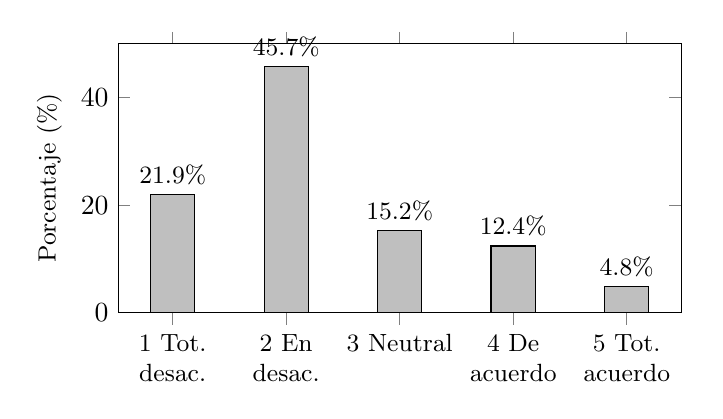
\begin{tikzpicture}
\begin{axis}[
  ybar,
  width=0.72\textwidth, height=5cm,
  bar width=16pt,
  ymin=0, ymax=50,
  ylabel={Porcentaje (\%)},
  xtick=data,
  symbolic x coords={1 Tot.\\desac., 2 En\\desac., 3 Neutral, 4 De\\acuerdo, 5 Tot.\\acuerdo},
  x tick label style={align=center, text width=1.5cm, font=\small},
  nodes near coords={\pgfmathprintnumber[fixed,precision=1]{\pgfplotspointmeta}\%},
  nodes near coords align={vertical},
  every node near coord/.style={font=\small},
  enlarge x limits=0.12,
  ylabel style={font=\small},
]
\addplot[fill=gray!50] coordinates {
  (1 Tot.\\desac., 21.9)
  (2 En\\desac.,    45.7)
  (3 Neutral,      15.2)
  (4 De\\acuerdo,   12.4)
  (5 Tot.\\acuerdo, 4.8)
};
\end{axis}
\end{tikzpicture}
\end{center}

\begin{center}
\renewcommand{\arraystretch}{1.25}
\begin{tabular}{|l|c|c|}
\hline
\textbf{Opción} & \textbf{Frecuencia} & \textbf{Porcentaje} \\ \hline
Totalmente en desacuerdo & 23 & 21{,}9\,\% \\ \hline
En desacuerdo & 48 & 45{,}7\,\% \\ \hline
Neutral & 16 & 15{,}2\,\% \\ \hline
De acuerdo & 13 & 12{,}4\,\% \\ \hline
Totalmente de acuerdo & 5 & 4{,}8\,\% \\ \hline
\textbf{Total} & \textbf{105} & \textbf{100{,}0\,\%} \\ \hline
\end{tabular}
\end{center}

\smallskip
El 67{,}6\,\% de los pacientes (en desacuerdo o totalmente en desacuerdo) considera que
\emph{no} le resultó fácil encontrar un horario disponible, frente a solo el 17{,}2\,\% que
lo percibe como sencillo. Esto refleja la saturación del canal de agendamiento manual.

\medskip
\textbf{Pregunta 2: Cuando escribo a la clínica por WhatsApp, la respuesta suele tardar más de lo que esperaría.}

\begin{center}
\begin{tikzpicture}
\pie[text=legend, radius=2, color={gray!20, gray!40, gray!60, gray!80, gray!100}]{5.7/Tot. desac., 7.6/En desac., 26.7/Neutral, 45.7/De acuerdo, 14.3/Tot. acuerdo}
\end{tikzpicture}
\end{center}

\begin{center}
\renewcommand{\arraystretch}{1.25}
\begin{tabular}{|l|c|c|}
\hline
\textbf{Opción} & \textbf{Frecuencia} & \textbf{Porcentaje} \\ \hline
Totalmente en desacuerdo & 6 & 5{,}7\,\% \\ \hline
En desacuerdo & 8 & 7{,}6\,\% \\ \hline
Neutral & 28 & 26{,}7\,\% \\ \hline
De acuerdo & 48 & 45{,}7\,\% \\ \hline
Totalmente de acuerdo & 15 & 14{,}3\,\% \\ \hline
\textbf{Total} & \textbf{105} & \textbf{100{,}0\,\%} \\ \hline
\end{tabular}
\end{center}

\smallskip
El 60{,}0\,\% de los pacientes está de acuerdo o totalmente de acuerdo en que la respuesta
por WhatsApp tarda más de lo esperado, corroborando la saturación operativa reportada por
la secretaria en el Instrumento~2.

\medskip
\textbf{Pregunta 3: En alguna ocasión he olvidado o confundido el día u hora de una cita.}

\begin{center}
\begin{tikzpicture}
\pie[text=legend, radius=2, color={gray!20, gray!40, gray!60, gray!80, gray!100}]{7.6/Tot. desac., 6.7/En desac., 17.1/Neutral, 53.3/De acuerdo, 15.2/Tot. acuerdo}
\end{tikzpicture}
\end{center}

\begin{center}
\renewcommand{\arraystretch}{1.25}
\begin{tabular}{|l|c|c|}
\hline
\textbf{Opción} & \textbf{Frecuencia} & \textbf{Porcentaje} \\ \hline
Totalmente en desacuerdo & 8 & 7{,}6\,\% \\ \hline
En desacuerdo & 7 & 6{,}7\,\% \\ \hline
Neutral & 18 & 17{,}1\,\% \\ \hline
De acuerdo & 56 & 53{,}3\,\% \\ \hline
Totalmente de acuerdo & 16 & 15{,}2\,\% \\ \hline
\textbf{Total} & \textbf{105} & \textbf{100{,}0\,\%} \\ \hline
\end{tabular}
\end{center}

\smallskip
El 68{,}5\,\% ha olvidado o confundido alguna vez el día u hora de su cita, dato que
evidencia la necesidad de un sistema de recordatorios automáticos.

\medskip
\textbf{Pregunta 4: Me habría evitado un problema si hubiera recibido un recordatorio automático antes de la cita.}

\begin{center}
\begin{tikzpicture}
\pie[text=legend, radius=2, color={gray!20, gray!40, gray!60, gray!80, gray!100}]{9.5/En desac., 26.7/Neutral, 56.2/De acuerdo, 7.6/Tot. acuerdo}
\end{tikzpicture}
\end{center}

\begin{center}
\renewcommand{\arraystretch}{1.25}
\begin{tabular}{|l|c|c|}
\hline
\textbf{Opción} & \textbf{Frecuencia} & \textbf{Porcentaje} \\ \hline
Totalmente en desacuerdo & 0 & 0{,}0\,\% \\ \hline
En desacuerdo & 10 & 9{,}5\,\% \\ \hline
Neutral & 28 & 26{,}7\,\% \\ \hline
De acuerdo & 59 & 56{,}2\,\% \\ \hline
Totalmente de acuerdo & 8 & 7{,}6\,\% \\ \hline
\textbf{Total} & \textbf{105} & \textbf{100{,}0\,\%} \\ \hline
\end{tabular}
\end{center}

\smallskip
El 63{,}8\,\% de los pacientes considera que un recordatorio automático le habría evitado
un problema, sin ningún paciente totalmente en desacuerdo. Esto respalda la funcionalidad
de notificación automática como la más valorada por la muestra.

\medskip
\textbf{Pregunta 5: Estaría dispuesto a agendar o reprogramar una cita mediante un asistente automatizado por WhatsApp.}

\begin{center}
\begin{tikzpicture}
\pie[text=legend, radius=2, color={gray!20, gray!40, gray!60, gray!80, gray!100}]{7.6/Tot. desac., 14.3/En desac., 15.2/Neutral, 50.5/De acuerdo, 12.4/Tot. acuerdo}
\end{tikzpicture}
\end{center}

\begin{center}
\renewcommand{\arraystretch}{1.25}
\begin{tabular}{|l|c|c|}
\hline
\textbf{Opción} & \textbf{Frecuencia} & \textbf{Porcentaje} \\ \hline
Totalmente en desacuerdo & 8 & 7{,}6\,\% \\ \hline
En desacuerdo & 15 & 14{,}3\,\% \\ \hline
Neutral & 16 & 15{,}2\,\% \\ \hline
De acuerdo & 53 & 50{,}5\,\% \\ \hline
Totalmente de acuerdo & 13 & 12{,}4\,\% \\ \hline
\textbf{Total} & \textbf{105} & \textbf{100{,}0\,\%} \\ \hline
\end{tabular}
\end{center}

\smallskip
El 62{,}9\,\% está de acuerdo o totalmente de acuerdo en agendar o reprogramar citas
mediante un asistente automatizado. Es la función de mayor demanda entre las tres evaluadas.

\medskip
\textbf{Pregunta 6: Estaría dispuesto a consultar precios o formas de pago mediante un asistente automatizado.}

\begin{center}
\begin{tikzpicture}
\pie[text=legend, radius=2, color={gray!20, gray!40, gray!60, gray!80, gray!100}]{4.8/Tot. desac., 14.3/En desac., 18.1/Neutral, 53.3/De acuerdo, 9.5/Tot. acuerdo}
\end{tikzpicture}
\end{center}

\begin{center}
\renewcommand{\arraystretch}{1.25}
\begin{tabular}{|l|c|c|}
\hline
\textbf{Opción} & \textbf{Frecuencia} & \textbf{Porcentaje} \\ \hline
Totalmente en desacuerdo & 5 & 4{,}8\,\% \\ \hline
En desacuerdo & 15 & 14{,}3\,\% \\ \hline
Neutral & 19 & 18{,}1\,\% \\ \hline
De acuerdo & 56 & 53{,}3\,\% \\ \hline
Totalmente de acuerdo & 10 & 9{,}5\,\% \\ \hline
\textbf{Total} & \textbf{105} & \textbf{100{,}0\,\%} \\ \hline
\end{tabular}
\end{center}

\medskip
\textbf{Pregunta 7: Estaría dispuesto a consultar horarios de atención mediante un asistente automatizado.}

\begin{center}
\begin{tikzpicture}
\pie[text=legend, radius=2, color={gray!20, gray!40, gray!60, gray!80, gray!100}]{6.7/Tot. desac., 9.5/En desac., 15.2/Neutral, 51.4/De acuerdo, 17.1/Tot. acuerdo}
\end{tikzpicture}
\end{center}

\begin{center}
\renewcommand{\arraystretch}{1.25}
\begin{tabular}{|l|c|c|}
\hline
\textbf{Opción} & \textbf{Frecuencia} & \textbf{Porcentaje} \\ \hline
Totalmente en desacuerdo & 7 & 6{,}7\,\% \\ \hline
En desacuerdo & 10 & 9{,}5\,\% \\ \hline
Neutral & 16 & 15{,}2\,\% \\ \hline
De acuerdo & 54 & 51{,}4\,\% \\ \hline
Totalmente de acuerdo & 18 & 17{,}1\,\% \\ \hline
\textbf{Total} & \textbf{105} & \textbf{100{,}0\,\%} \\ \hline
\end{tabular}
\end{center}

\smallskip
En los tres ítems de la sección, el porcentaje de acuerdo o total acuerdo supera el
60\,\%. La disposición más alta corresponde a la consulta de horarios (68{,}5\,\%), seguida
de agendar citas (62{,}9\,\%) y consultar precios (62{,}8\,\%), lo que confirma la viabilidad
de adopción de un asistente automatizado por parte de la mayoría de la muestra.

\medskip
\textbf{Pregunta 8: ¿A través de qué canal coordinó su última cita en Bellidental?}

\medskip
\begin{center}
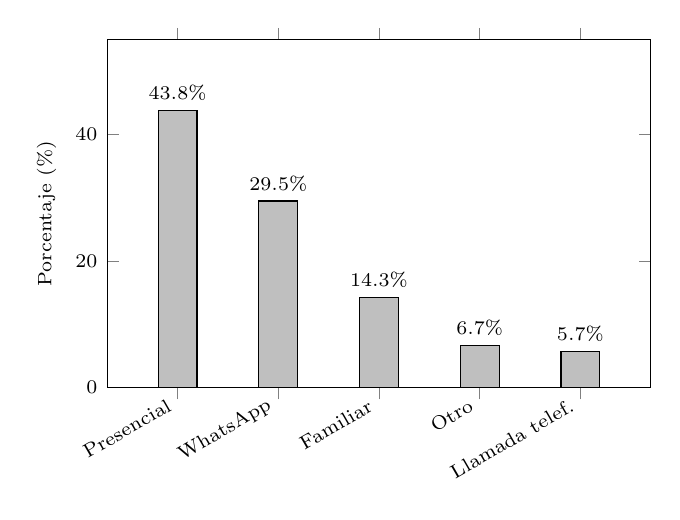
\begin{tikzpicture}
\begin{axis}[
  ybar,
  width=0.7\linewidth, height=6cm,
  bar width=14pt,
  ymin=0, ymax=55,
  ylabel={Porcentaje (\%)},
  xtick={1,2,3,4,5},
  xticklabels={Presencial, WhatsApp, Familiar, Otro, Llamada telef.},
  x tick label style={rotate=30, anchor=east, font=\scriptsize},
  xmin=0.3, xmax=5.7,
  nodes near coords={\pgfmathprintnumber[fixed,precision=1]{\pgfplotspointmeta}\%},
  nodes near coords align={vertical},
  every node near coord/.style={font=\scriptsize},
  tick label style={font=\scriptsize},
  ylabel style={font=\scriptsize},
]
\addplot[fill=gray!50] coordinates {
  (1, 43.8)
  (2, 29.5)
  (3, 14.3)
  (4, 6.7)
  (5, 5.7)
};
\end{axis}
\end{tikzpicture}
\end{center}

\bigskip
\begin{center}
\renewcommand{\arraystretch}{1.25}
\begin{tabular}{|l|r|r|}
\hline
\textbf{Canal} & \textbf{n} & \textbf{\%} \\ \hline
Presencial en recepción & 46 & 43{,}8 \\ \hline
WhatsApp                & 31 & 29{,}5 \\ \hline
Por un familiar         & 15 & 14{,}3 \\ \hline
Otro                    & 7  &  6{,}7 \\ \hline
Llamada telefónica      & 6  &  5{,}7 \\ \hline
\textbf{Total}          & \textbf{105} & \textbf{100{,}0} \\ \hline
\end{tabular}
\end{center}

\smallskip
El canal presencial en recepción fue el más frecuente (43{,}8\,\%), seguido por WhatsApp
(29{,}5\,\%). La suma de canales digitales y telefónicos (WhatsApp + llamadas = 35{,}2\,\%)
indica una demanda significativa de atención no presencial que un agente automatizado
podría absorber.
